\chapter[Otimização multiobjetivo]{Otimização multiobjetivo}

A otimização multiobjetivo consiste em selecionar as melhores soluções de acordo com múltiplos critérios ao invés de apenas um. Por exemplo, ao estabelecer um melhor caminho entre duas cidades pode-se não estar interessado apenas na menor distância, mas também no tráfego, segurança das vias, quantidade de pedágios, etc. A otimização de apenas um objetivo é simples, para que uma solução seja considerada melhor que a outra, basta que ela tenha uma melhor avaliação. Por outro lado, quando se trabalha com mais de uma função de otimização, é preciso usar o conceito de dominância de Pareto.

A dominância de Pareto diz que uma solução $A$ é melhor que uma solução $B$, ou $A$ domina $B$ ($A \prec B$), se, e somente se:

\begin{itemize}  
	\item $A$ é melhor avaliado que $B$ em pelo menos um dos objetivos;
	\item $A$ não tem avaliação pior que $B$ em nenhum dos objetivos.
\end{itemize}

Considerando um problema de minimização e $F$ como o conjunto de funções objetivo, tem-se, matematicamente:

\[A \prec B \Leftrightarrow (\forall(f \in F) f(A) \leq f(B)) \land (\exists (f \in F) f(A) < f(B))\]

Em problemas de otimização multiobjetivo, o interesse está em encontrar o conjunto de todas as soluções que não são dominadas por nenhuma outra, ou seja, a fronteira de Pareto. Graficamente, a fronteira de Pareto representa a linha formada pelas soluções não-dominadas existentes para o problema. Na figura \ref{fig_pareto} apresenta-se um exemplo de uma fronteira de Pareto para um problema de minimização com dois objetivos ($F1$ e $F2$), a fronteira de Pareto está representada em vermelho. Observe que nenhum círculo vermelho possui ambos F1 e F2 menores que alguma outra solução em vermelho, ou seja, são não-dominadas. Em contra-partida, toda solução acima da fronteira, em cinza, é dominada, pois existe alguma solução em vermelho que possui ambos valores de F1 e F2 menores. Caso o problema em questão fosse de maximização, a fronteira de Pareto estaria acima de qualquer solução não-dominada ao invés de abaixo.

\begin{figure}
	\label{fig_pareto}
	\caption{Fronteira de Pareto}
	\centering
	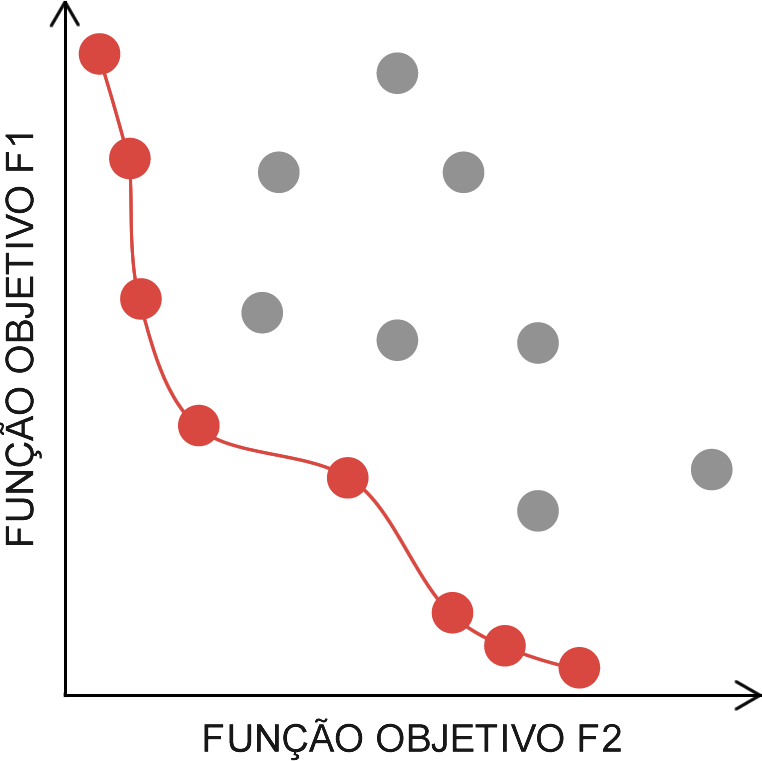
\includegraphics[width=0.4\textwidth]{cap_otimizacao-multi/figs/pareto}
\end{figure}

Não existe limite para o número de funções objetivo em um problema de otimização, mas quanto maior ele for, mais complexa é a busca. Os algoritmos clássicos de otimização multiobjetivo NSGA-II e SPEA2 lidam bem com até dois objetivos, mas a partir de quatro critério de otimização, ambos os métodos sofrem para encontrar soluções relevantes. Desta forma, criou-se a classificação "many-objective". Problemas many-objectives (4 ou mais objetivos) apresentam diversas novas dificuldades e precisam de novas técnicas para que sejam resolvidos eficientemente. Como observado por Deb em [nsga3], os problemas trazidos pelo alto número de objetivos são:

\begin{enumerate}  
	\item Grande parte da população é não dominada: a maioria dos algoritmos multiobjetivos classifica a população de acordo com a dominação de Pareto. Se existem muitas funções objetivo, se torna muito comum que uma solução seja melhor que outra em pelo menos uma das funções. Desta forma, a maior parte das soluções se torna não-dominada, o que impede os algoritmos de evoluírem a população, já que todos os indivíduos são considerados igualmente bons.
	\item Avaliar a diversidade da população se torna computacionalmente caro: afim de garantir uma boa diversidade populacional, alguns algoritmos medem alguma espécie de distância entre as soluções e removem as que são consideradas mais similares. A maior dimensionalidade traz consequentemente um maior impacto no cálculo da proximidade entre os indivíduos. 
	\item Crossover ineficiente: a alta dimensionalidade do espaço de busca faz com que os indivíduos na população sejam muito distante uns dos outros e, normalmente, o cruzamento entre duas soluções muito diferentes resultam num filho muito distante dos pais, o que prejudica a convergência da busca. Portanto, pode ser necessário redefinir os operadores de recombinação afim de restringir as possibilidades de pareamento.
	\item População demasiadamente grande: quanto maior o número de objetivos, maior o número de soluções na fronteira de Pareto, portanto, para obter-se bons resultados, é necessário que se manipule grandes populações de indivíduos, o que é computacionalmente caro e dificulta o trabalho do usuário que deverá escolher uma única solução ao final do processo.
	\item Métricas de avaliação se tornam difíceis de se calcular: a avaliação das soluções está diretamente relacionada ao número de objetivos, quanto maior ele for, maior será o esforço computacional necessário. A complexidade do hiper-volume, por exemplo, cresce exponencialmente com o número de objetivos.
	\item Dificuldade de visualização: é fácil representar graficamente as soluções e a fronteira de Pareto em problemas de até três objetivos. Com 4 funções em diante, se torna difícil tal visualização.
\end{enumerate}

A maior parte dos algoritmos many-objectives (todos mencionados neste trabalho) lidam apenas com os três primeiros problemas. Sobre a quarta dificuldade fazemos um breve estudo mais adiante [citar seção] e as duas últimas não são responsabilidade dos algoritmos de otimização em sí.

\section{Algoritmos Multiobjetivo}

\subsection{Non-dominated Sorting Genetic Algorithm II (NSGA-II)}
O NSGA-II [] é o algoritmo evolutivo multiobjetivo (AEMO) mais frequente na literatura. A atribuição de aptidão (fitness) se dá pela classificação da população em rankings de dominância (fronteiras), de forma que o primeiro contenha todas as soluções não dominadas, o segundo todos os indivíduos não-dominados excluindo a primeira fronteira, e assim por diante. Quanto melhor o ranking de uma solução, melhor sua aptidão e  maior sua chance de sobreviver para a próxima geração. Várias soluções, pertencem à mesma fronteira, a fim de diferenciá-las utiliza-se um cálculo de distância (crowding distance), o qual confere melhor avaliação às soluções mais diferenciadas umas das outras, garantindo assim a diversidade da população.

O processo do NSGA-II é semelhante ao do algoritmo genético comum, com diferença no cálculo de aptidão, que é feito por ranks, e no cálculo de distâncias, que é inexistente na proposta original do AG. O primeiro passo continua sendo a geração aleatória dos indivíduos, em seguida classifica-se a população em ranks de dominância e inicia-se o laço principal, o qual termina assim que a condição de parada é atingida. O laço principal do NSGA-II é dado pelo pseudo-código do algoritmo \ref{alg_nsgaii}.

\begin{algorithm}
	\caption{Laço principal do NSGA-II}
	\label{alg_nsgaii}
	\begin{algorithmic}[1]
		\While {número máximo de gerações não for atingido}
		\State selecione os pares de pais para o crossover
		\State efetue o cruzamento para cada par de pais, gerando os filhos
		\State combine a população de pais com a população de filhos
		\State classifique todas as soluções em fronteiras (ranks) de dominância 
		\State calcule a crowding distance para cada uma das soluções
		\State aplique a seleção natural sobre a totalidade da população, preservando os indivíduos de melhor rank e, em segundo lugar, crowding distance.
		\EndWhile
	\end{algorithmic}
\end{algorithm}

A seleção de pais utiliza torneio simples para sorteá-los, ou seja, dois elementos da população são escolhidos de forma aleatória, o indivíduo com melhor avaliação é selecionado como um dos pais, sorteia-se mais dois indivíduos, e o melhor dentre eles se torna o segundo pai.

Na linha 2 do pseudo-código, através dos pares de pais, gera-se os filhos através do crossover e da mutação. Após a geração dos filhos, a população corrente e o conjunto de filhos são concatenados (linha 3) e submetidos à classificação em ranks de dominância (linha 4).

A classificação em ranks de dominância recebe um conjunto de soluções e verifica quais dentre elas não são dominadas. O conjunto de soluções não dominadas forma o primeiro rank de dominância. Do conjunto restante (excluindo o primeiro rank), retira-se as soluções não dominadas para formar o segundo rank. Esse processo se repete até que todos os indivíduos tenham sido classificados.

Após toda a população ter sido classificada em ranks, antes de selecionar os indivíduos que vão compor a população na próxima iteração, deve-se calcular a distância de aglomeração (crowding distance) para cada indivíduo em cada rank de dominância. O cálculo de distância, para cada objetivo, ordena o conjunto de soluções e faz uma relação entre as distâncias de cada indivíduo para os vizinhos imediatamente anterior e posterior. Soma-se as distâncias obtidas em cada objetivo para cada solução e define-se aquelas com maior valor de distância como as mais diferentes entre sí.

Com toda a população classificada em ranks e todas as distâncias calculadas, basta formar a nova população com os melhores indivíduos. Para isso, analisa-se fronteira a fronteira, da melhor para a pior, até que o tamanho máximo da população seja atingido. Para cada fronteira aplica-se o seguinte processo de decisão:

\begin{itemize}  
	\item Se $tamanho(rank) + tamanho(nova_população) < tam_max_pop$: adiciona-se todos os membros do rank à nova população.
	\item Caso contrário, se $tamanho(nova_população) < tam_max_pop$: adiciona-se à nova população os $tam_max_pop - tamanho(nova_população)$ elementos do rank com os maiores valores de distância. Termine o processo, a nova população está formada.
	\item Caso contrário, termine o processo, a nova população está formada.
\end{itemize}

Desta forma, ao final do algoritmo obtém-se a fronteira de Pareto aproximada no primeiro rank da população gerada na última iteração do algoritmo.

\subsection{Strength Pareto evolutionary algorithm 2 (SPEA2)}

O SPEA2 é um AEMO que calcula, para cada membro da população, sua força (strength) e densidade. A força de uma solução é dada pelo número de indivíduos que ela domina, enquanto a densidade é uma medida de distância para os vizinhos mais próximos, quanto maior a densidade mais próximo o indivíduo está das demais soluções. A aptidão (fitness) de uma solução é definida por sua densidade mais a soma das forças de todo indivíduo que a domina. As principais diferenças entre o SPEA2 e um AG comum estão no cálculo de aptidão e na utilização de uma população extra: o arquivo.

O arquivo é responsável por guardar as melhores soluções já encontradas até o momento, funciona como uma espécie de elitismo. Os pais, no cruzamento, são sempre escolhidos do arquivo e os filhos substituem 100\% da população corrente. A cada iteração, os melhores indivíduos entre a população e o arquivo compõe o arquivo da geração seguinte. A quantidade de indivíduos no repositório de soluções não-dominadas é limitada e, portanto, quando se excede o tamanho máximo, deve-se executar um processo de truncamento.

O processo de truncamento do arquivo ocorre na seleção natural, a última função executada na iteração do laço principal de um AG. A seleção no SPEA2 se dá pelo cálculo do arquivo da próxima geração: ambas as populações da iteração corrente (população e arquivo) são submetidas à seleção, extrai-se do conjunto total de soluções aquelas que não são dominadas por nenhuma outra e com esse subconjunto ($n_d$) constrói-se o novo arquivo através do seguinte processo de decisão:

\begin{itemize}  
	\item Se $tamanho(n_d) = capacidade\_arquivo$, o novo arquivo é formado por $n_d$;
	\item Caso contrário, se $tamanho(n_d) < capacidade\_arquivo$, o novo arquivo é formado pela união de $n_d$ com os $capacidade\_arquivo - tamanho(n_d)$ indivíduos restantes com melhor aptidão;
	\item Caso contrário, se $tamanho(n_d) > capacidade\_arquivo$, o novo arquivo é formado por $n_d$ e deve-se truncá-lo em $tamanho(n_d) - capacidade\_arquivo$ passos, onde em cada passo elimina-se o indivíduo com menor variabilidade genética em relação aos demais.
\end{itemize}

Os indivíduos mais aptos no SPEA2 são aqueles dominados pela menor quantidade de soluções e que possuem maior variabilidade genética. O algoritmo calcula a aptidão em três etapas: cálculo de força (\textit{strength}), do \textit{raw fitness} e densidade.

A força de um indivíduo $i$ ($s(i)$) é o número de soluções que ele domina, ou seja, considerando $E$ o arquivo e $P$ a população:

\[ s(i) = |j|: j \in P \cup E \land i \prec j \]

Tendo calculado a força de cada indivíduo, parte-se para o \textit{raw fitness}. O \textit{raw fitness} de um indivíduo $i$ ($r(i)$) é dado pela soma das forças de cada elemento que o domina. Veja a fórmula a seguir:

\[ r(i) = \sum_{j \in E \cup P | j \prec i} s(j) \]

Observe que, caso o indivíduo seja não-dominado, seu \textit{raw fitness} será o menor possível: zero. Após determinar o \textit{raw fitness}, para finalizar o cálculo de aptidão deve-se descobrir a densidade de cada indivíduo ($d(i)$). A densidade é computada de acordo com a distância da solução para seus vizinhos e é dada pela seguinte fórmula:

\[ d(i) = \frac{1}{\sigma_i^k + 2} \]

Na fórmula acima, $\sigma_i^k$ é a k-ésima menor distância entre o indivíduo $i$ e o restante da população. k é a raiz quadrada do tamanho do conjunto de soluções em avaliação, i.e. $k = \sqrt{|P \cup E|}$. O valor de $d(i)$ sempre está no intervalo (0,1). Referencia-se o leitor ao artigo original do SPEA2 [] para mais detalhes sobre o cálculo de densidade.

Finalmente, a aptidão do indivíduo ($f(i)$) é dada pela soma do \textit{raw fitness} e a densidade: $f(i) = r(i) + d(i)$. Como, $\forall i, d(i) < 1$ e, $\forall i, r(i) = 0$ se a solução é não-dominada, $f(i) < 1$ sempre que $i$ é não-dominado.

O laço principal do SPEA2 é explicitado no pseudo-código \ref{alg_spea2} e como resposta para o problema, retorna-se o arquivo da última geração computada. Espera-se que, após as diversas iterações, o algoritmo tenha conseguido uma boa aproximação da fronteira de Pareto.

\begin{algorithm}
	\caption{Laço principal do SPEA2}
	\label{alg_spea2}
	\begin{algorithmic}[1]
		\While {número máximo de gerações não for atingido}
		\State a partir do arquivo, selecione os pares de pais para o crossover
		\State efetue o cruzamento para cada par de pais, gerando os filhos
		\State substitua a população corrente pelos filhos
		\State calcule o fitness de todos indivíduos no arquivo e na população
		\State aplique a seleção natural e trunque o arquivo, caso necessário
		\EndWhile
	\end{algorithmic}
\end{algorithm}

\section{Algoritmos Many-objectives}

\subsection{Multiobjective evolutionary algorithm based on decomposition (MOEA/D)}

O MOEA/D é um algoritmo que avalia os objetivos através de uma função escalarizadora, se baseando na dominância de Pareto apenas para atualizar o conjunto de soluções não dominadas geradas em cada iteração (arquivo). No MOEA/D, um problema multiobjetivo é decomposto em múltiplos problemas mono-objetivos chamados de células. Cada célula é definida por um vetor de pesos gerado aleatoriamente e representa um indivíduo, ou seja, o número de células é igual ao tamanho da população. Além dos pesos, a célula, ou indivíduo, é composta de uma solução e uma vizinhança. A vizinhança é formada pelos $k$ indivíduos mais próximos de acordo com o vetor de pesos, onde $k$ é um parâmetro do algoritmo que representa o tamanho das vizinhanças. A aptidão (fitness) de uma solução é calculada de acordo com sua avaliação em cada objetivo, a função escalarizadora, e o vetor de pesos da célula. Em toda geração, uma nova solução é gerada para cada célula, onde a vizinhança é levada em consideração para a escolha do pai e seleção natural.

O primeiro passo do MOEA/D é gerar a estrutura de células e vizinhanças, para isso, sorteia-se os vetores de pesos (a soma de cada vetor deve ser igual a um) e para cada um deles, calcula-se os $k$ vetores mais próximos (vizinhança). Essa estrutura é imutável e é utilizada no decorrer de todo o algoritmo. A geração dos vetores de pesos pode ser tanto aleatória quanto seguir uma distribuição pré-definida. Antes de começar o laço principal, gera-se aleatoriamente uma solução para cada célula e calcula-se as aptidões. 

Uma parte fundamental do MOEA/D é a escolha da função escalarizadora, ela é a principal responsável pelo cálculo de aptidão. Em todos experimentos realizados neste trabalho, foi utilizada a soma ponderada, mas outras estratégia como \textit{Penalty-Based Boundary Intersection} e Tchebycheff também podem ser utilizadas [moead]. A aptidão de uma solução é calculada através da função escalarizadora e do vetor de pesos, por exemplo, se os valores $[2, 9, 5]$ representam a solução $s$ no espaço de objetivos, $[0.3, 0.2, 0.5]$ é o vetor de pesos da célula $c$, e a soma ponderada é a função escalarizadora, então a aptidão de $s$ em $c$ é dada por $2 * 0.3 + 9 * 0.2 + 5 * 0.5 = 4.9$.

No laço principal do MOEA/D, seleciona-se os pais e gera-se os filhos. Para cada célula $c_i$, dois pais são selecionados aleatoriamente em sua vizinhança. Sempre que um filho é gerado, o processo de seleção é realizado logo em seguida. A aptidão do filho é calculada para cada uma das células na vizinhança de $c_i$, substituindo a solução anterior da célula caso seu fitness seja melhor. Após o processo de geração de filhos e seleção, atualiza-se o arquivo com as soluções novas soluções não-dominadas.

\subsection{Non-dominated Sorting Genetic Algorithm III (NSGA-III)}

O NSGA-III é uma extensão do NSGA-II que permite o \textit{framework} funcionar melhor para mais de três objetivos. Ele se diferencia do original apenas na fase de seleção, onde ao invés de usar a distância de aglomeração para diferenciar soluções em uma mesma fronteira, utiliza um método de clusterização, onde os indivíduos são divididos em nichos de acordo com suas similaridades. O NSGA-III é caracterizado pelo processo de atribuição de nicho chamado de classificação não-dominada baseada em pontos de referência. Sua ideia é traçar uma figura geométrica de uma dimensão a menos que o número de objetivos nos pontos extremos da primeira fronteira. Um número pré-definido de pontos de referência equidistantes é distribuído sobre a figura e passa a representar cada um, um nicho. Para classificar uma solução, define-se como nicho o ponto de referência mais próximo. Ao final, toma-se como sobreviventes os pontos nas regiões menos lotadas do espaço de busca. Para mais detalhes sobre o processo de clusterização, referencia-se o leitor ao artigo original [NSGA-III].

\subsection{Algoritmo Evolutivo Multiobjetivo com Muitas Tabelas (AEMMT)}

O AEMMT, assim como o MOEA/D, decompõe o problema multiobjetivo em subproblemas menores e para isso utiliza um esquema de tabelas, onde cada tabela representa uma combinação diferente de objetivos. A função que transforma os múltiplos objetivos em um valor escalar é sempre a média e cada tabela mantém os melhores indivíduos considerando a média dos objetivos que representa. A cada geração, duas tabelas são selecionadas para o cruzamento. Dois pais, um de cada tabela, são sorteados aleatoriamente para gerarem um único filho, que será testado em todas as tabelas, entrando naquelas em que representar uma melhor aptidão em relação aos demais indivíduos. Naturalmente, como um único \textit{crossover} é realizado a cada iteração, o AEMMT precisa de mais gerações para efetuar o mesmo número de comparações que os algoritmos citados nas seções anteriores.

A quantidade de tabelas é determinada pelo número de combinações possíveis de objetivos. Para quatro objetivos ($f_1, f_2, f_3, f_4$), por exemplo, como ilustrado na figura \ref{fig_aemmt_tabelas} serão criadas 15 tabelas de combinações mais uma tabela extra, usada para guardar os indivíduos não-dominados.

\begin{figure}
	\label{fig_aemmt_tabelas}
	\caption{Tabelas do AEMMT}
	\centering
	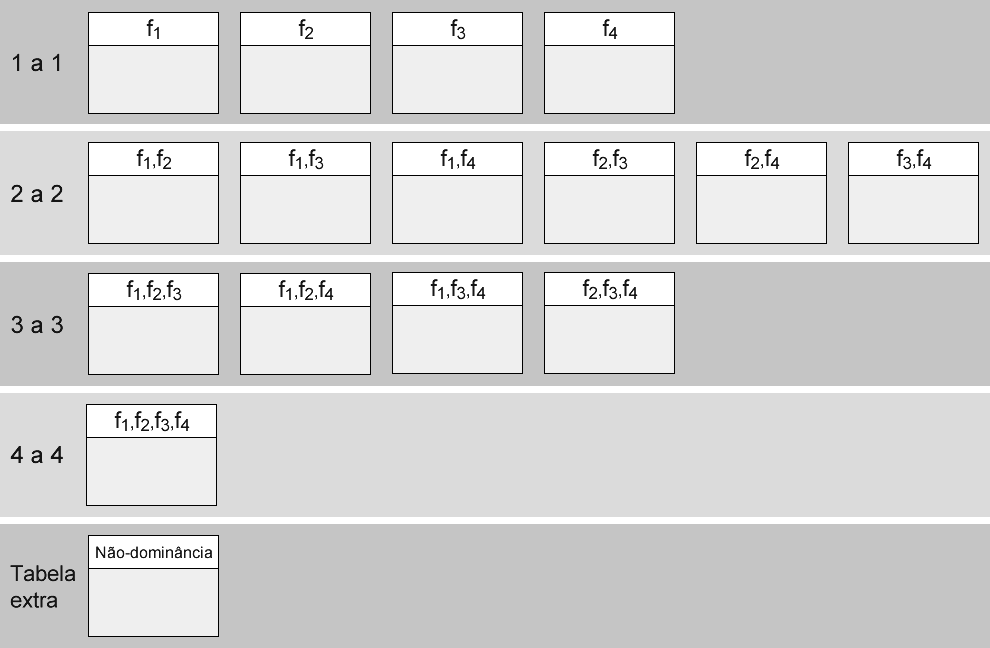
\includegraphics[width=1\textwidth]{cap_otimizacao-multi/figs/aeemt-tabelas}
\end{figure}

Cada tabela possui um limite máximo de indivíduos e no início do algoritmo gera-se soluções aleatórias de forma que todas as tabelas sejam completamente preenchidas. No laço principal, um indivíduo só entra em uma tabela $t$ se for melhor que a pior solução na população de $t$. Com relação a tabela de dominância, sempre que um filho é gerado e não-dominado por nenhum outro indivíduo na tabela, ele é incluído. A restrição no tamanho da tabela de dominância é independente das demais e sempre que o limite for atingido, é feito um truncamento priorizando a permanência das soluções com maior valor de média aritmética entre todos os objetivos.

O primeiro passo do AEMMT é gerar as tabelas e preenchê-las com soluções aleatórias. Em seguida, inicia-se o laço principal, onde em cada iteração são escolhidas duas tabelas vai torneio duplo de acordo com suas pontuações. A pontuação tem valor inicial zero e sempre que uma tabela gera um filho que sobrevive para a geração seguinte, sua pontuação é incrementada. As pontuações são zeradas a cada 100 gerações. Considerando as duas tabelas que vencem os torneios, sorteia-se um indivíduo de cada e efetua-se o cruzamento entre os dois. O filho gerado é então comparado tabela à tabela, entrando naquelas em que representar uma melhoria. Após a execução de todas as gerações, espera-se que a população da tabela extra de não-dominância tenha convergido para a fronteira de Pareto.

\subsection{Algoritmo Evolutivo Multiobjetivo com Múltiplas Dominâncias (AEMMD)}

O AEMMD é uma modificação do AEMMT que, apesar de usar o mesmo processo de de divisão do problema multi-objetivo, abandona a ideia de escalarização e volta a utilizar o conceito de dominância dos métodos mais antigos (e.g. NSGA-II e SPEA2). No AEMMD, ao invés de se utilizar a média dos objetivos da tabela para avaliar o indivíduo, lança-se mão da relação de dominância de Pareto, um indivíduo novo $s$ só entra na tabela $t$, se $s$ não for dominado por nenhuma solução em $t$. Além disso, se $s$ entra em $t$, todas as soluções em $t$ dominadas por $s$ são removidas.

